
\begin{figure*}[ht!]
	\centering
	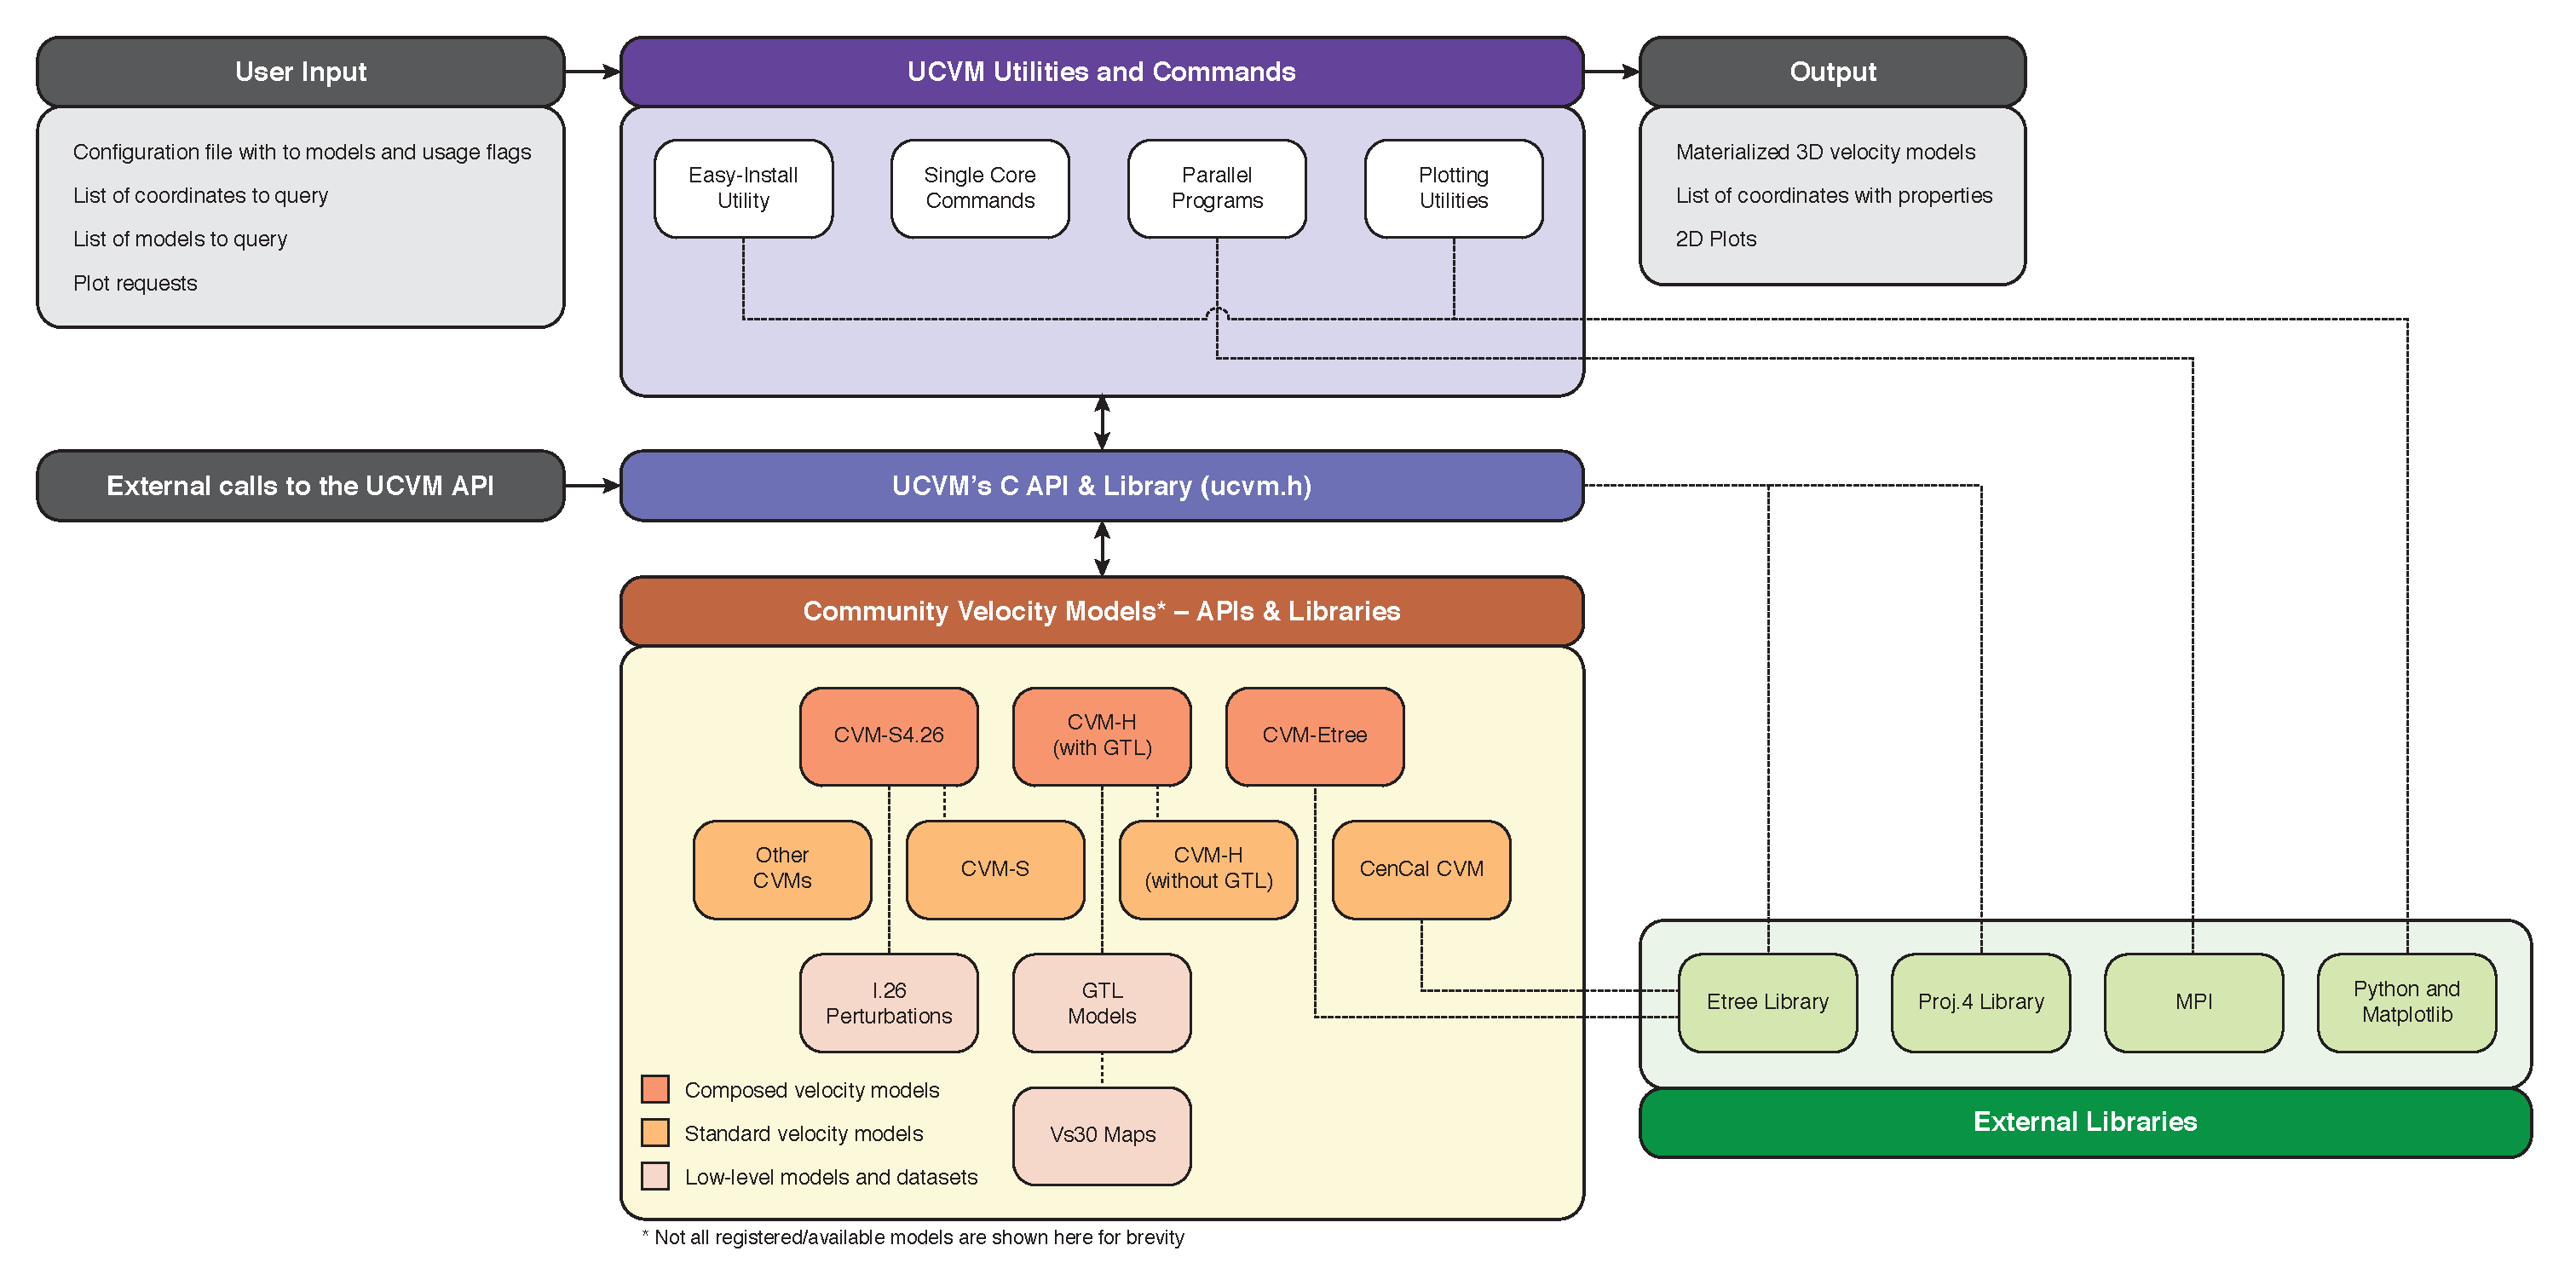
\includegraphics
		[width=\textwidth]
		{figures/pdf/ucvm-sw-architecture}
	\caption{The UCVM software architecture. Gray-colored frames indicate components at the level of user or client interaction. The upper purple-colored frame displays UCVM utilities and commands directly accessible to users, whereas the ligher purpled-colored box indicates the lower-level UCVM API and library upon which UCVM operations rest. Underlying this, are a selection of community models supported by UCVM; and to the right, in green, are the library dependencies of the UCVM framework. Here we distinguish models and datasets in four categories related to their origin or operational concept. In practice, however, UCVM treats each model or dataset independently and without any distinction.}
	\label{fig:sw.arch}
\end{figure*}
